\documentclass{beamer}
\title{The Effects of Rotation on Stratified Turbulence}
%\author[Dante Buhl]{Dante Buhl {\scriptsize Advised by: Pascale Garaud, Hongyun Wang}}
\date{November 25, 2024}
\institute{UCSC Applied Mathematics}
\graphicspath{ {./images/} }
\usepackage{verbatim}
\usetheme{Dresden}
%\usecolortheme{spruce}
\usecolortheme{dolphin}
\usefonttheme{serif}
\usepackage{amsmath}
\usepackage{pifont}
\usepackage{hyperref}
\usepackage{amsthm} %proof environment
\usepackage{amssymb}
\usepackage{amsfonts}
%\usepackage{enumitem} %nice lists
\usepackage{verbatim} %useful for something 
\usepackage{xcolor}
\usepackage{blindtext} % I have no idea what this is 
\usepackage{caption}  % need this for unnumbered captions/figures
\usepackage{soul} % need this for the hl command
\usepackage{graphicx} % Required for inserting images
\usepackage{multimedia}
\usepackage{natbib}

\begin{document}

\newcommand{\wrms}{w_{\text{rms}}}
\newcommand{\bs}[1]{\boldsymbol{#1}}
\newcommand{\tb}[1]{\textbf{#1}}
\newcommand{\bmp}[1]{\begin{minipage}{#1\textwidth}}
\newcommand{\emp}{\end{minipage}}
\newcommand{\R}{\mathbb{R}}
\newcommand{\C}{\mathbb{C}}
\newcommand{\N}{\mathcal{N}}
\newcommand{\K}{\bs{\mathrm{K}}}
\newcommand{\m}{\bs{\mu}_*}
\newcommand{\s}{\bs{\Sigma}_*}
\newcommand{\dt}{\Delta t}
\newcommand{\dx}{\Delta x}
\newcommand{\tr}[1]{\text{Tr}(#1)}
\newcommand{\Tr}[1]{\text{Tr}(#1)}
\newcommand{\Div}{\nabla \cdot}
\renewcommand{\div}{\nabla \cdot}
\newcommand{\Curl}{\nabla \times}
\newcommand{\Grad}{\nabla}
\newcommand{\grad}{\nabla}
\newcommand{\grads}{\nabla_s}
\newcommand{\gradf}{\nabla_f}
\newcommand{\xs}{\bs{x}_s}
\newcommand{\xf}{\bs{x}_f}
\newcommand{\ts}{t_s}
\newcommand{\tf}{t_f}
\newcommand{\pt}{\partial t}
\newcommand{\pz}{\partial z}
\newcommand{\uvec}{\bs{u}}
\newcommand{\F}{\bs{F}}
\newcommand{\T}{\tilde{T}}
\newcommand{\ez}{\bs{e}_z}
\newcommand{\ex}{\bs{e}_x}
\newcommand{\ey}{\bs{e}_y}
\newcommand{\eo}{\bs{e}_{\bs{\Omega}}}
\newcommand{\ppt}[1]{\frac{\partial #1}{\partial t}}
\newcommand{\ppts}[1]{\frac{\partial #1}{\partial t_s}}
\newcommand{\pptf}[1]{\frac{\partial #1}{\partial t_f}}
\newcommand{\ppz}[1]{\frac{\partial #1}{\partial z}}
\newcommand{\ddz}[1]{\frac{d #1}{d z}}
\newcommand{\ppzetas}[1]{\frac{\partial^2 #1}{\partial \zeta^2}}
\newcommand{\ppzs}[1]{\frac{\partial #1}{\partial z_s}}
\newcommand{\ppzf}[1]{\frac{\partial #1}{\partial z_f}}
\newcommand{\ppx}[1]{\frac{\partial #1}{\partial x}}
\newcommand{\ppy}[1]{\frac{\partial #1}{\partial y}}
\newcommand{\ppzeta}[1]{\frac{\partial #1}{\partial \zeta}}


\begin{comment}
    1. Intro 
    2. Model
        - new forcing mechanism
    3. Previous Work?
        - Multiscale theory by Chini et al and Shahe et al
    4. Stochastically forced Stratified TurbulenceA
        - new horizontal structures in the flow
        - weak correlation between vertical vorticity and mixing
        - previous wmrs scalings aren't as effective
    5. Rotating Stratified Turbulence
        - new flow structures (columns appear in the flow)
        - mixinng is localized to anti-cyclones
        - inverse energy cascade to small horizontal wavenumbers
        - decline in vertical mixing 
        
\end{comment}

\frame{\titlepage}

\section{Introduction}


\begin{frame}{Schematic}
    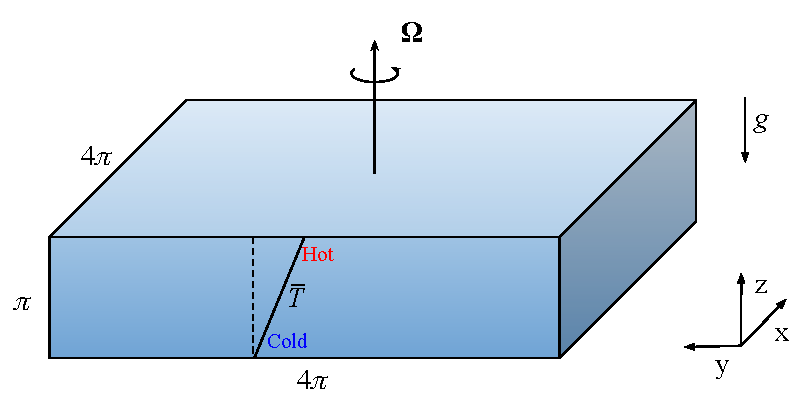
\includegraphics[width = \textwidth]{images/schematic.pdf}

    %\hl{add temp profile, gravity}
    % Notes: Tripply Periodic Domain with dimensions 4pi x 4pi x pi. We notice
    % the rotation vector omega placed in the diagram to visualize the angle of
    % rotation with respect to gravity (or the vertical coordinate direction).
    % It should also be noted that the rotation vector should be pointing in the
    % y direction. 
    % For the results you will be seeing today, rotation has not yet been
    % included, but it is the next step for our parameter study. 
\end{frame}

\begin{frame}{Governing Equations}

    {\small
    \begin{align}
        \ppt{\bs{u}} + \uvec \cdot \Grad \uvec +
        \frac{1}{Ro}(\ez \times
        \uvec) &= -\Grad p +
        \frac{T}{Fr^2}\ez + \F + \frac{1}{Re}\Grad^2\uvec \tag{mom.}\label{eq:momentum}\\
        \ppt{T} + \bs{u} \cdot \Grad T + w &= \frac{1}{Pe}\Grad^2T \tag{temp.} \label{eq:temp} \\
        \Div \bs{u} &= 0 \tag{cont.}\label{eq:cont}
    \end{align}}
    
    %\begin{align*}
        %Re = \frac{UL}{\nu}, \quad Pe = \frac{UL}{\kappa}, \quad Fr =
        %\frac{U}{NL}, \quad Ro = \frac{U}{2\Omega L}
    %\end{align*}
    %}
    %\begin{itemize}
        %\item $U$ is the characteristic velocity
        %\item $L$ is the large eddy horizontal length scale
        %\item $N$ is the buoyancy frequency ($N = \sqrt{\alpha_Tg\ddz{\bar{T}}}$)
        %\item $\Omega$ is the angular velocity
        %\item $(\nu, \kappa)$ are the (viscous, thermal) diffusivity coefficients
    %\end{itemize}
    %Where $U$ is the characteristic velocity, $L$ is the eddy length scale, $N$ is the buoyancy frequency, and $\Omega$ is the angular velocity of the rotating body. 
    % Notes: Classic Non-dimensionalized Boussinesue Rotations which include a
    % buopyancy field, viscous and dissipative dynamics, as well as rotation
    % (the coriolis force). Thus we see the appearnce of the Rossby, Froude,
    % Reynolds, and Peclet numbers in the governing equations. It should b
    % mentioned that this rotation vector r = <0, sin(\phi), cos(\phi)>. 

\end{frame}

\begin{frame}{Forcing Mechanism}

    We choose our forcing to be purely horizontal and divergence-free:
    \[
        \bs{F} = F_x\ex + F_y\ey, \quad \grad \cdot \uvec = 0
    \]
    The forcing is applied in spectral space and satisfies $\bs{k} \cdot \hat{\bs{F}} = 0$:
    \begin{gather*}
        \hat{F}_x = \frac{k_y}{|\bs{k}_h|}G(\bs{k}_h,t), \quad \hat{F}_y = \frac{-k_x}{|\bs{k}_h|}G(\bs{k}_h,t)\\
        G(\bs{k}_h,t) \in \C
    \end{gather*}
    where $G(\bs{k}_h,t)$ is a Gaussian process of amplitude 1 and correlation timescale 1. 

\end{frame}

% what are the flow structures that we obtain?
\begin{frame}{From Stratified Turbulence to rotationally domainated flow}
    % Ux rms figure
    % plot info: B100 is -3.5:3.5
    % B300 is -5:5
    % B10 is -3:3
    %B1 is -5:5
    \centering

    Typical non-rotating flows, properties of stratified turbulence


    \bmp{.235}
        \centering
        $1/Fr = 1$
        \vspace{2pt}
        
        %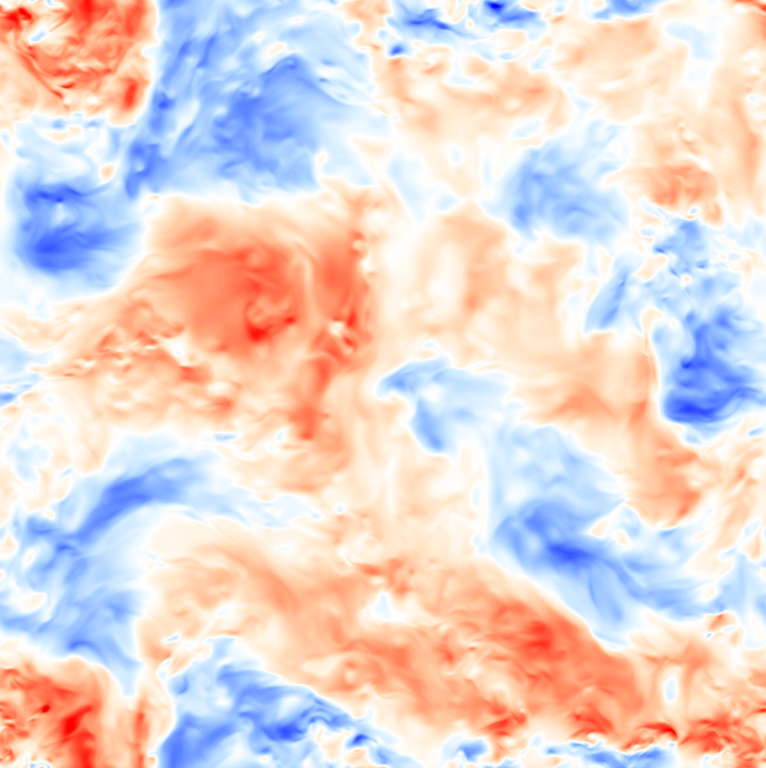
\includegraphics[width=\textwidth]{files/XYB1ux.png}
        %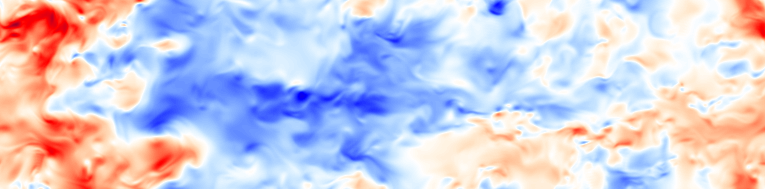
\includegraphics[width=\textwidth]{files/XZB1ux.png}
        %\includegraphics[width = \textwidth]{files/B1Spec.pdf}
    \emp
    \hspace{1pt}
    \bmp{.235}
        \centering
        $1/Fr = 3.16$
        \vspace{2pt}
        
        %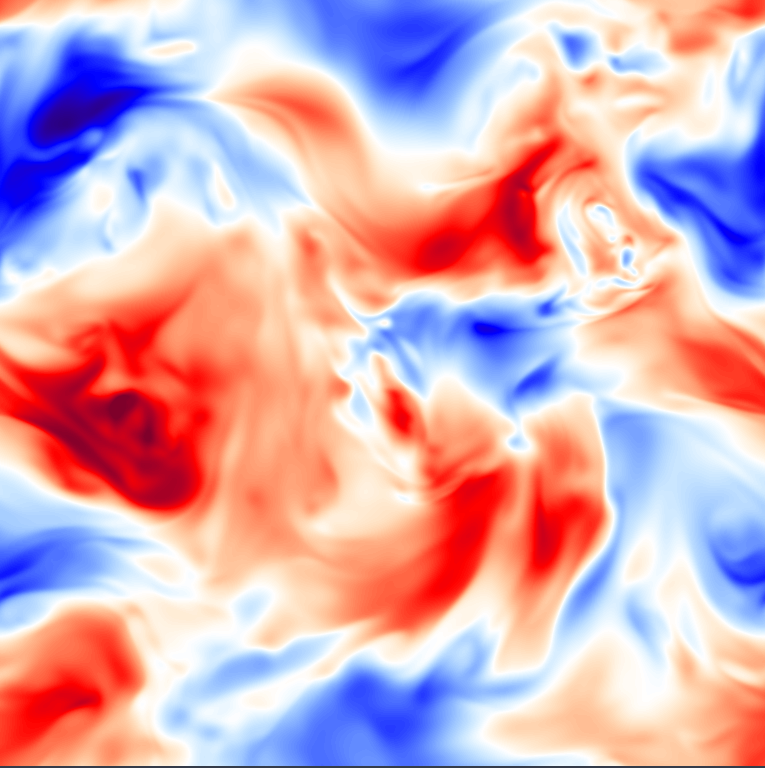
\includegraphics[width=\textwidth]{files/XYB10ux.png}
        %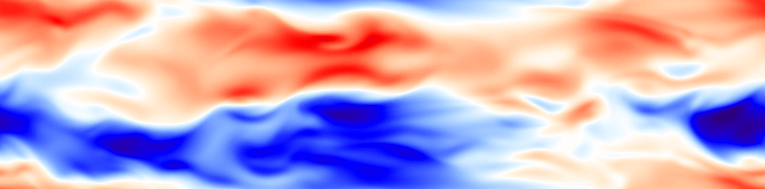
\includegraphics[width=\textwidth]{files/XZB10ux.png}
        %\includegraphics[width = \textwidth]{files/B10Spec.pdf}
    \emp
    \hspace{1pt}
    \bmp{.235}
        \centering
        $1/Fr = 10$
        \vspace{2pt}
        
        %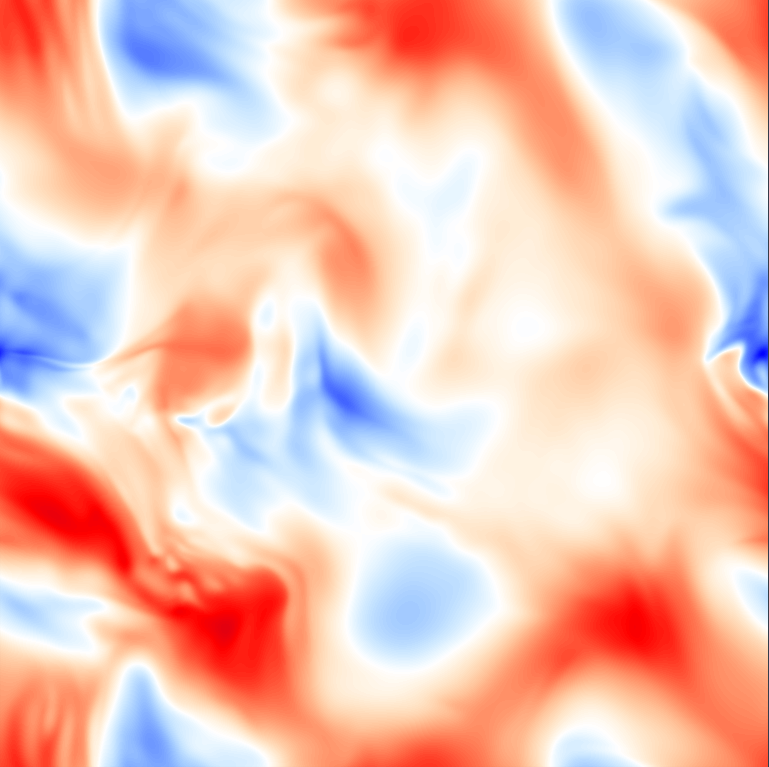
\includegraphics[width=\textwidth]{files/XYB100ux.png}
        %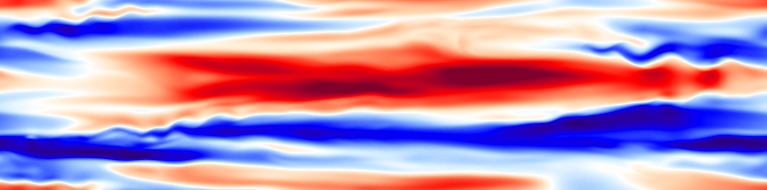
\includegraphics[width=\textwidth]{files/XZB100ux.png}
        %\includegraphics[width = \textwidth]{files/B100Spec.pdf}
    \emp
    \hspace{1pt}
    \bmp{.235}
        \centering
        $1/Fr = 17.36$
        \vspace{2pt}
        
        %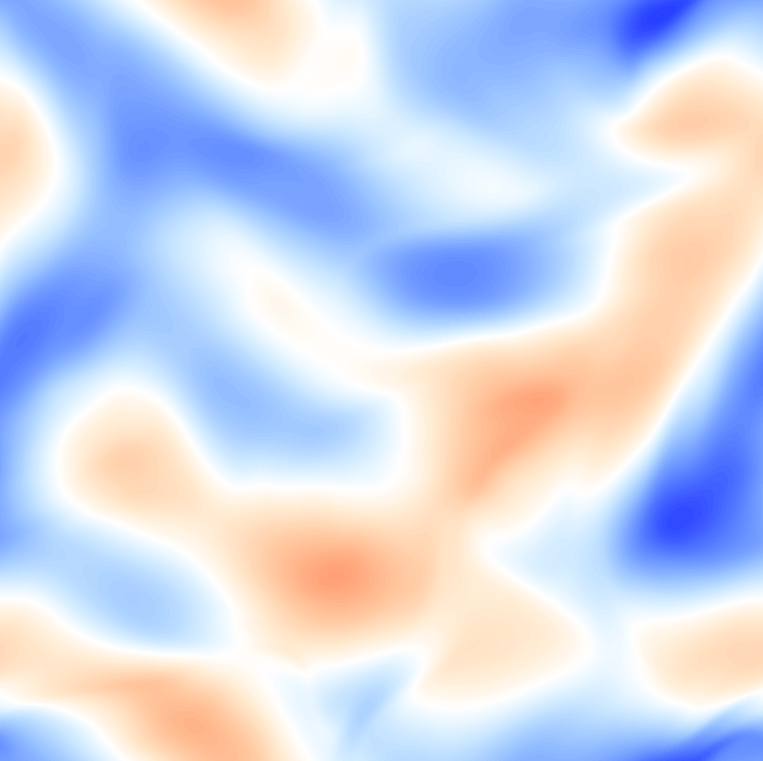
\includegraphics[width=.99\textwidth]{files/XYB300ux.png}
        %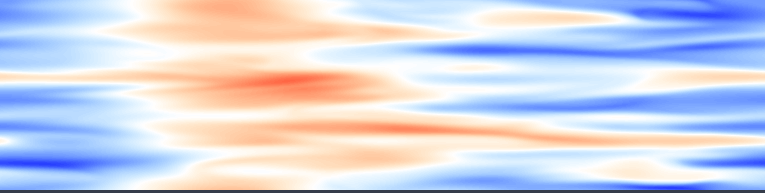
\includegraphics[width=.99\textwidth]{files/XZB300ux.png}
        %\includegraphics[width = \textwidth]{files/B300Spec.pdf}
    \emp
    \[\overrightarrow{\rm Stratification}\]
\end{frame}

\begin{frame}
    Increasing rotation, typical rotating flows
\end{frame}

% Energy Spectrum
\begin{frame}{Inverse Energy Cascade}

    \bmp{.33}
        \centering
        $Ro^{-1} = 1$
        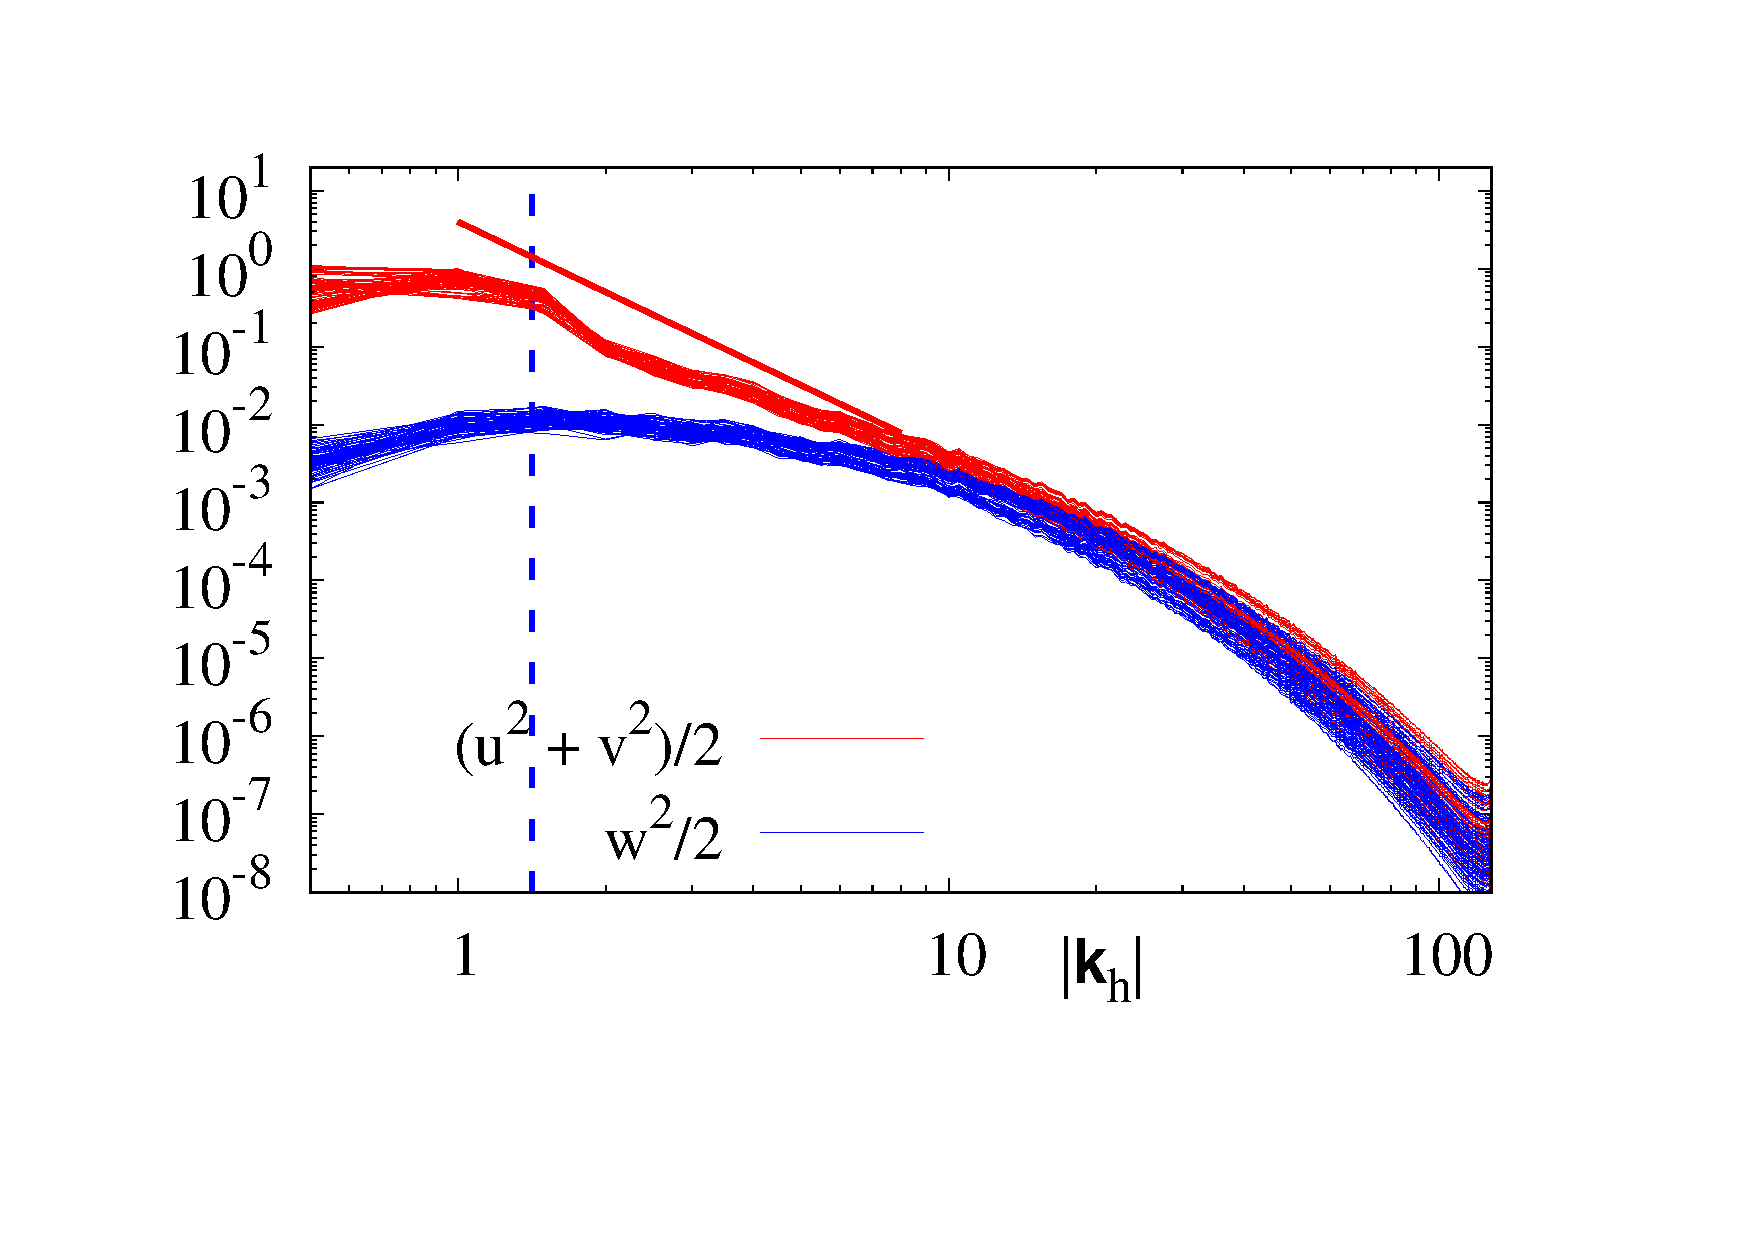
\includegraphics[width=\textwidth]{images/Om1Spec.pdf}
    \emp
    \bmp{.33}
        \centering
        $Ro^{-1} = 2$
        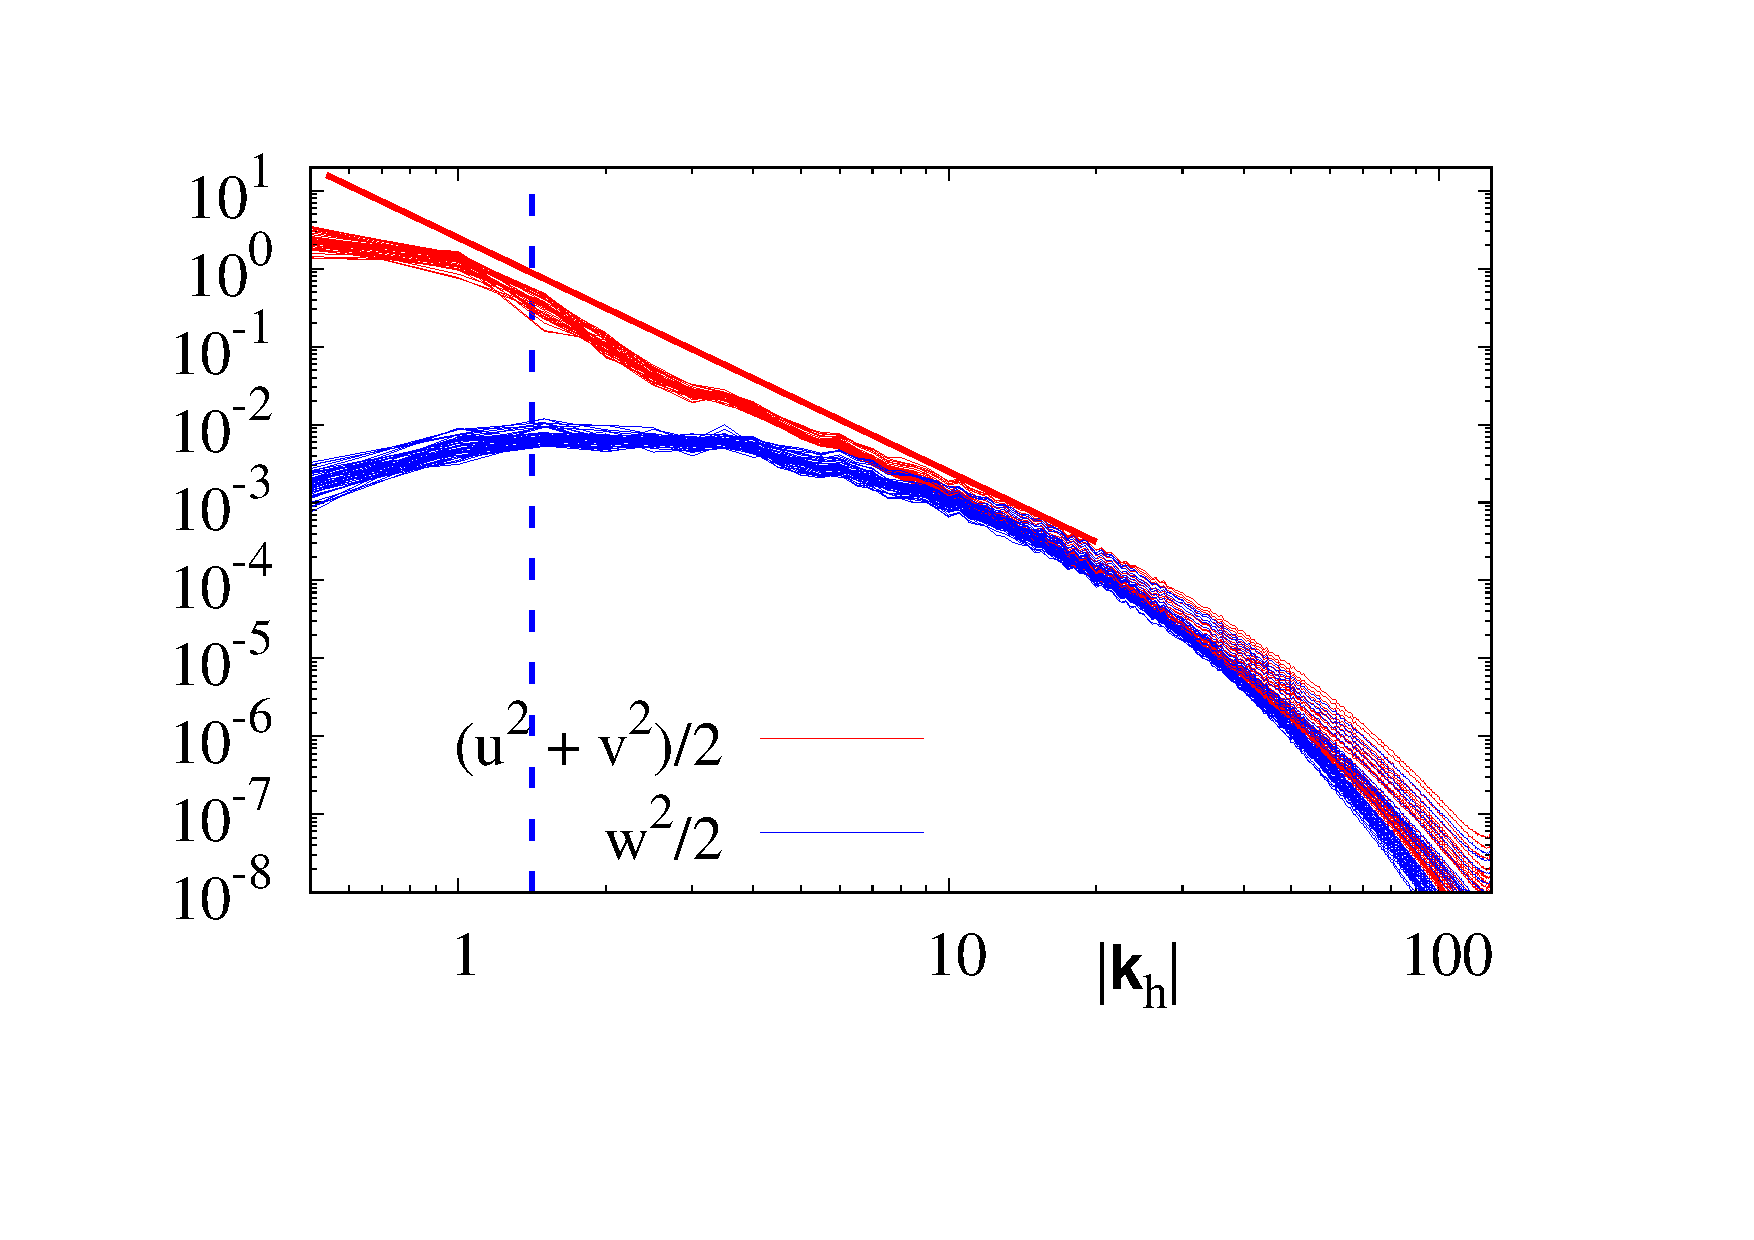
\includegraphics[width=\textwidth]{images/Om2Spec.pdf}
    \emp
    \bmp{.33}
        \centering
        $Ro^{-1} = 5$
        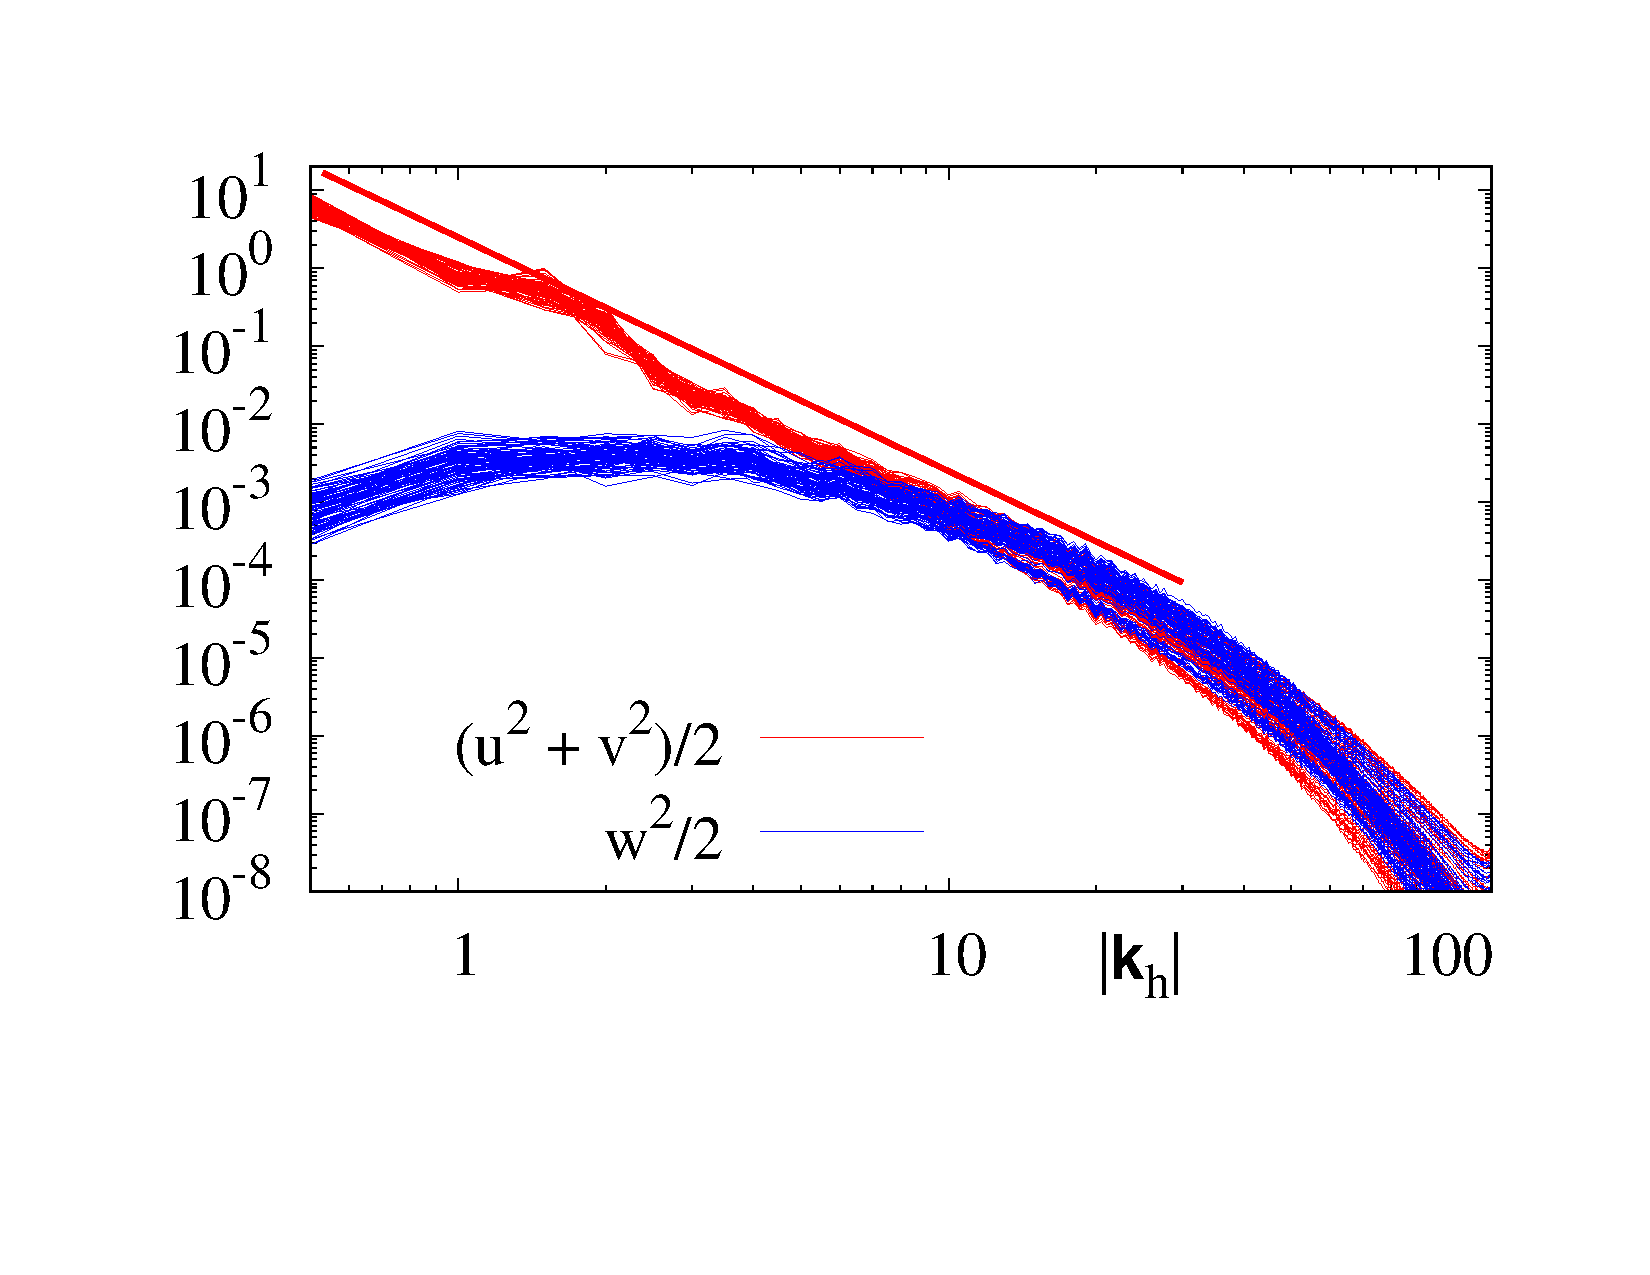
\includegraphics[width=\textwidth]{images/Om5Spec.pdf}
    \emp

\end{frame}
%RMS Data
\begin{frame}{R.M.S. Data}
    \bmp{.49}
        \centering
        %u_h 
        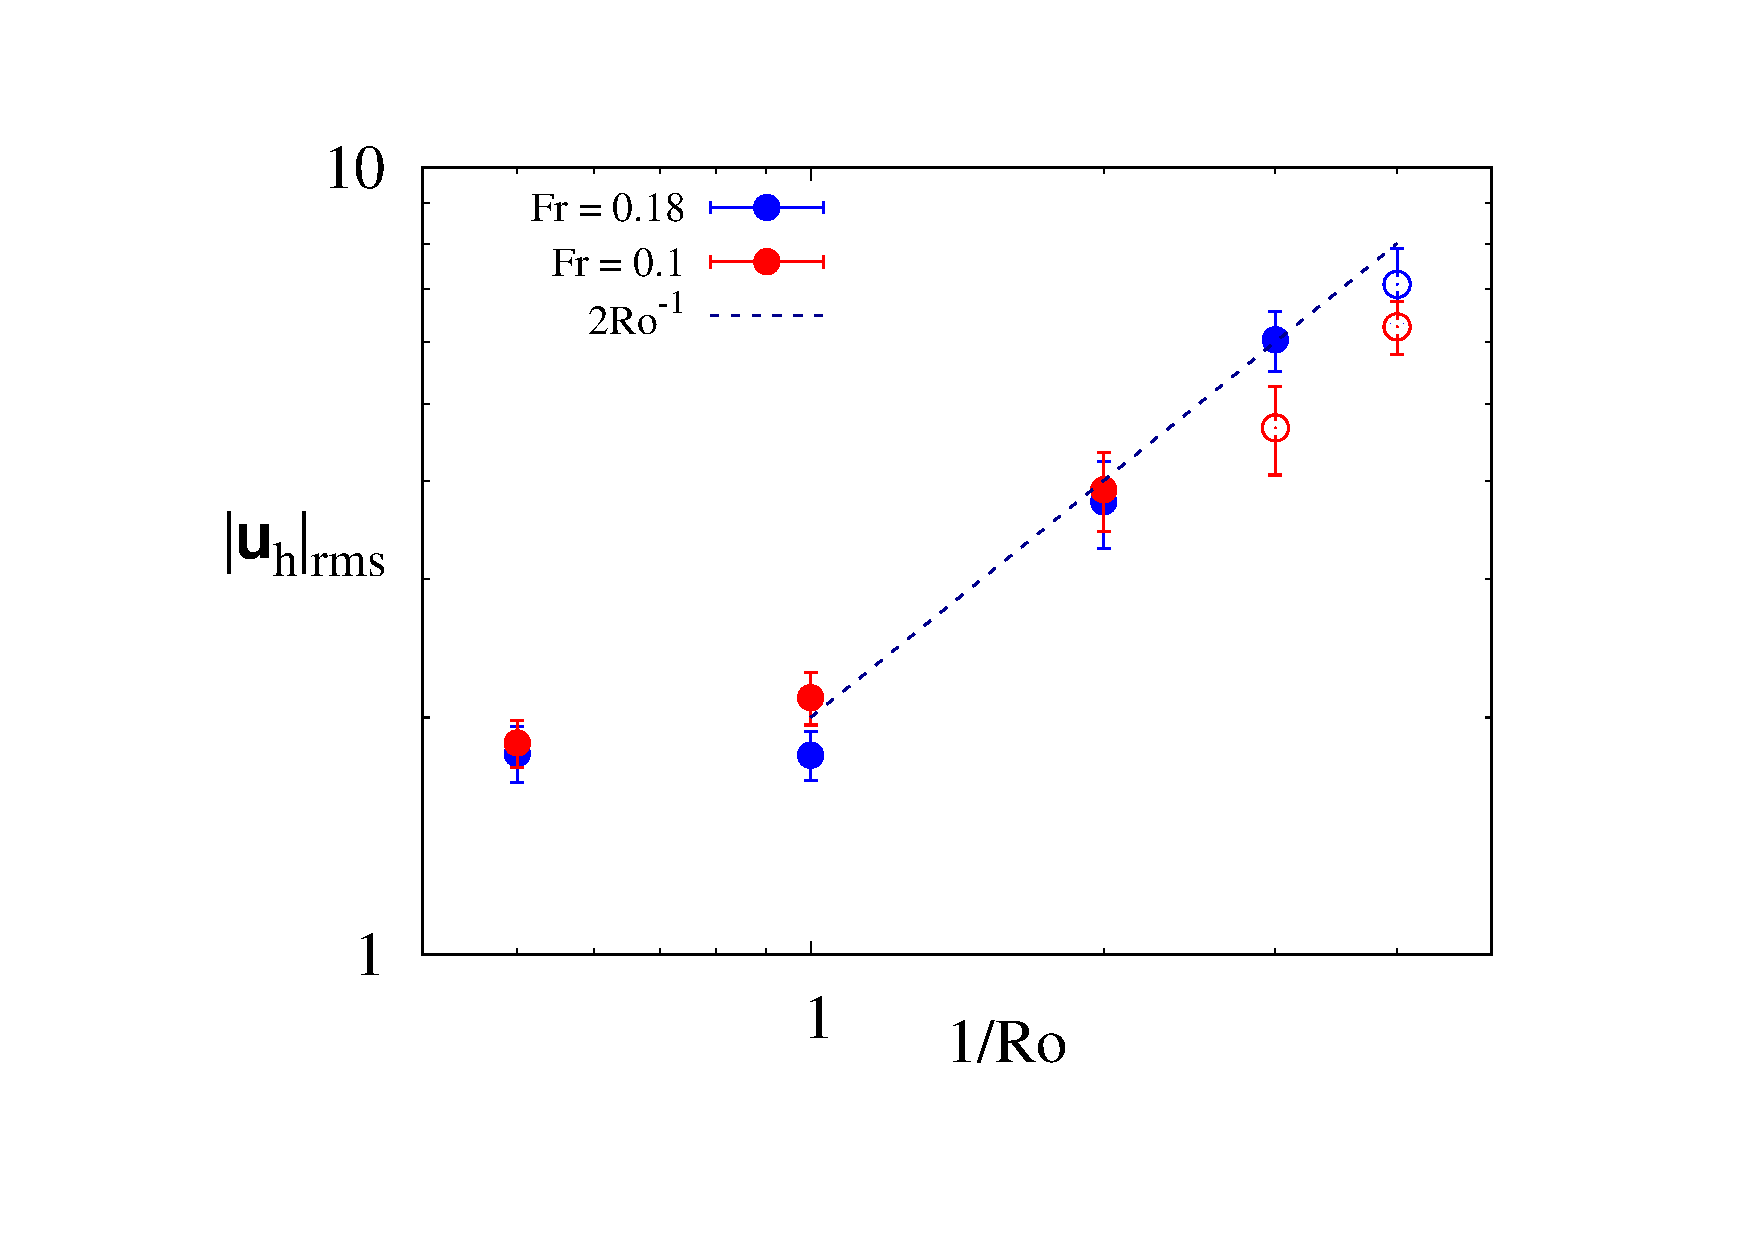
\includegraphics[width=1\textwidth]{images/urms_plot.pdf}
    \emp
    \bmp{.49}
        % w
        \centering
        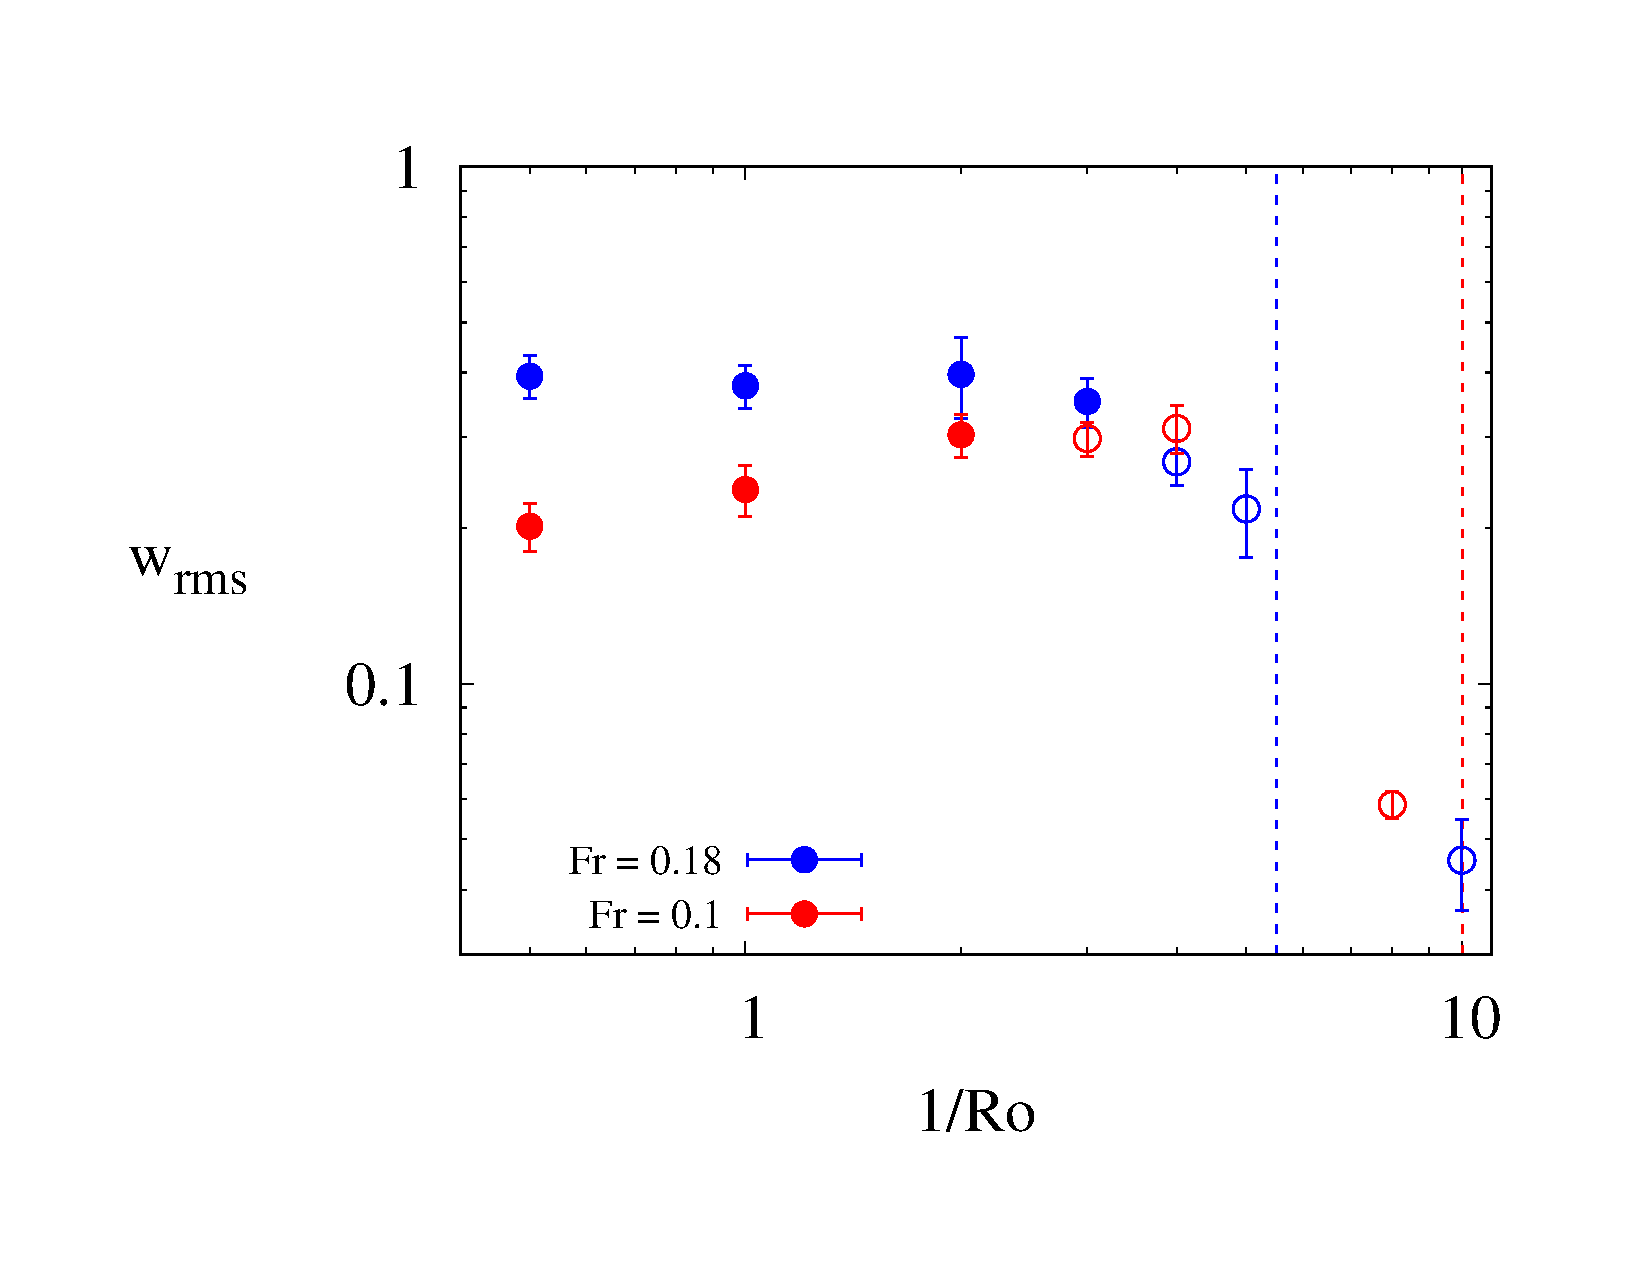
\includegraphics[width=1\textwidth]{images/wrms_plot.pdf}
    \emp
    
    \bmp{.49}
        % eta
        \centering
        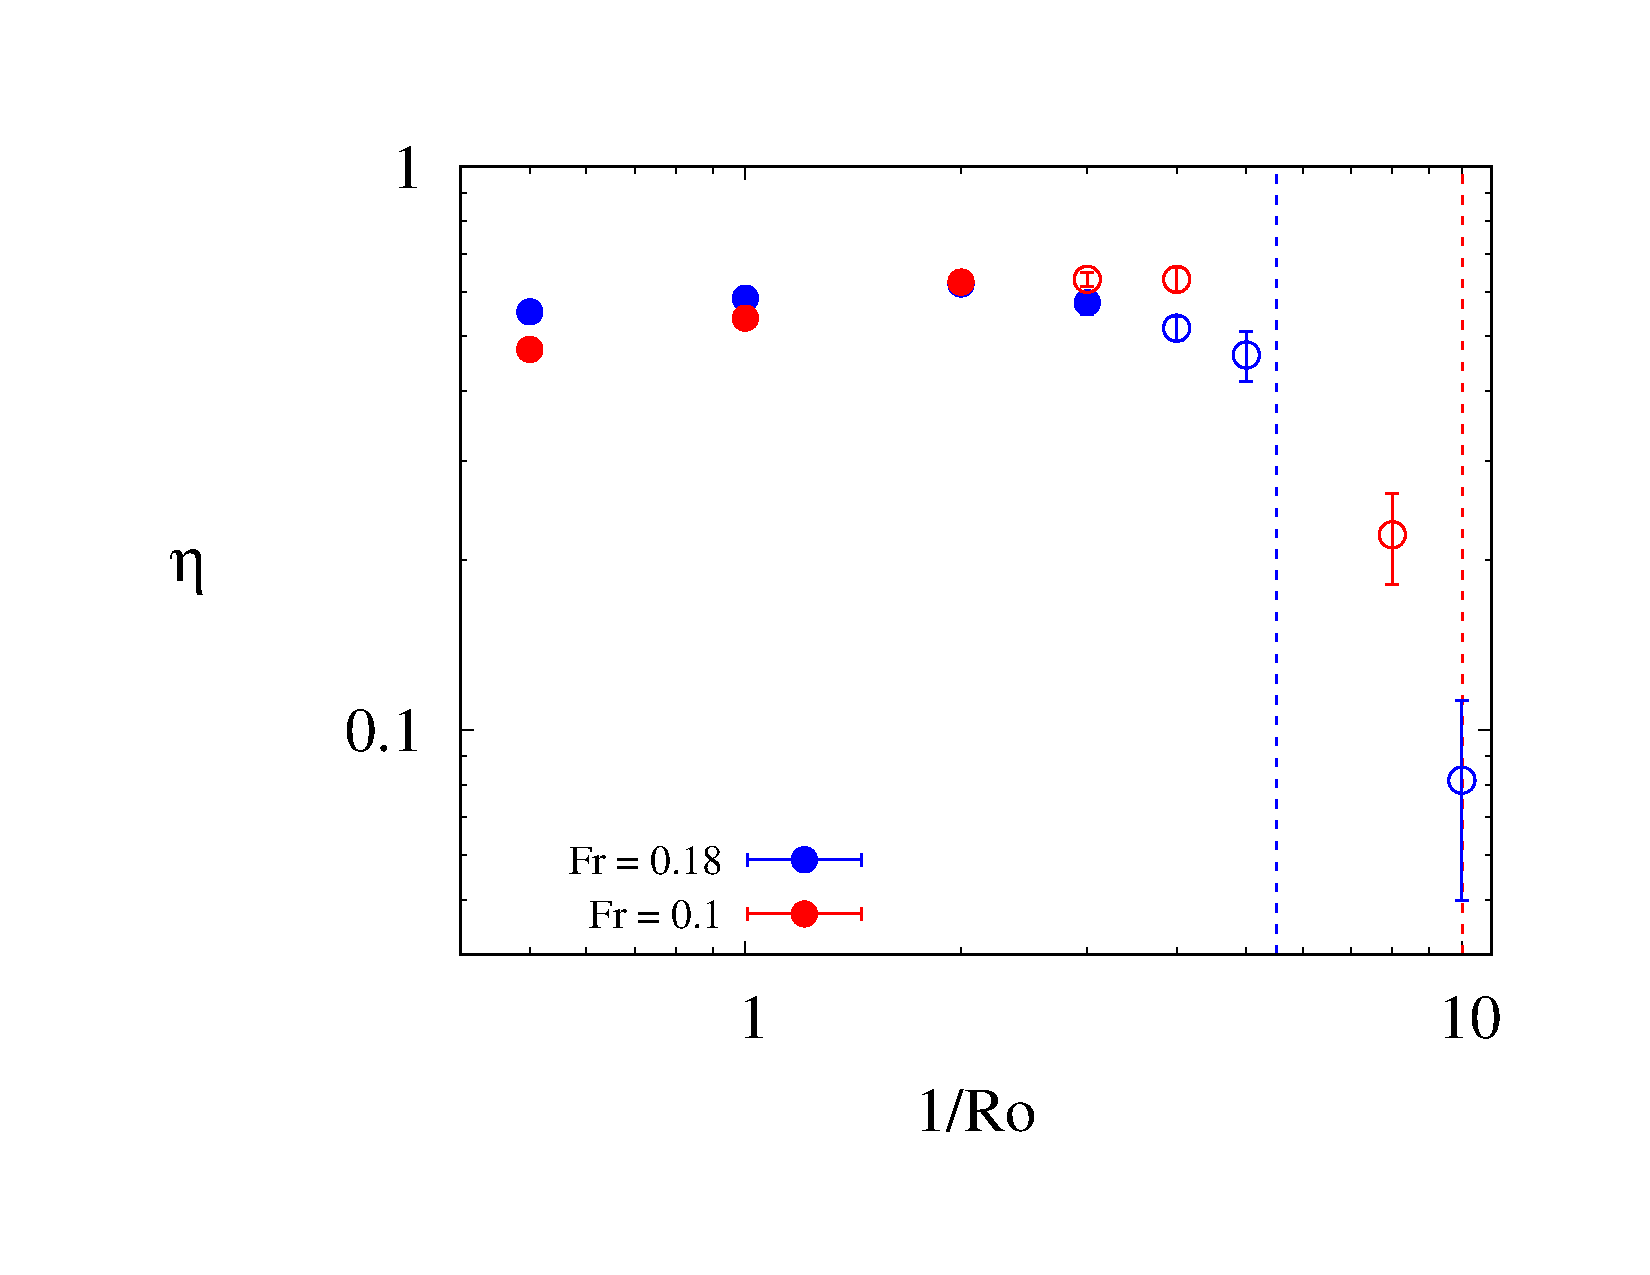
\includegraphics[width=1\textwidth]{images/mixing_plot.pdf}
    \emp
    \bmp{.49}
        % buoyancy flux
        \centering
        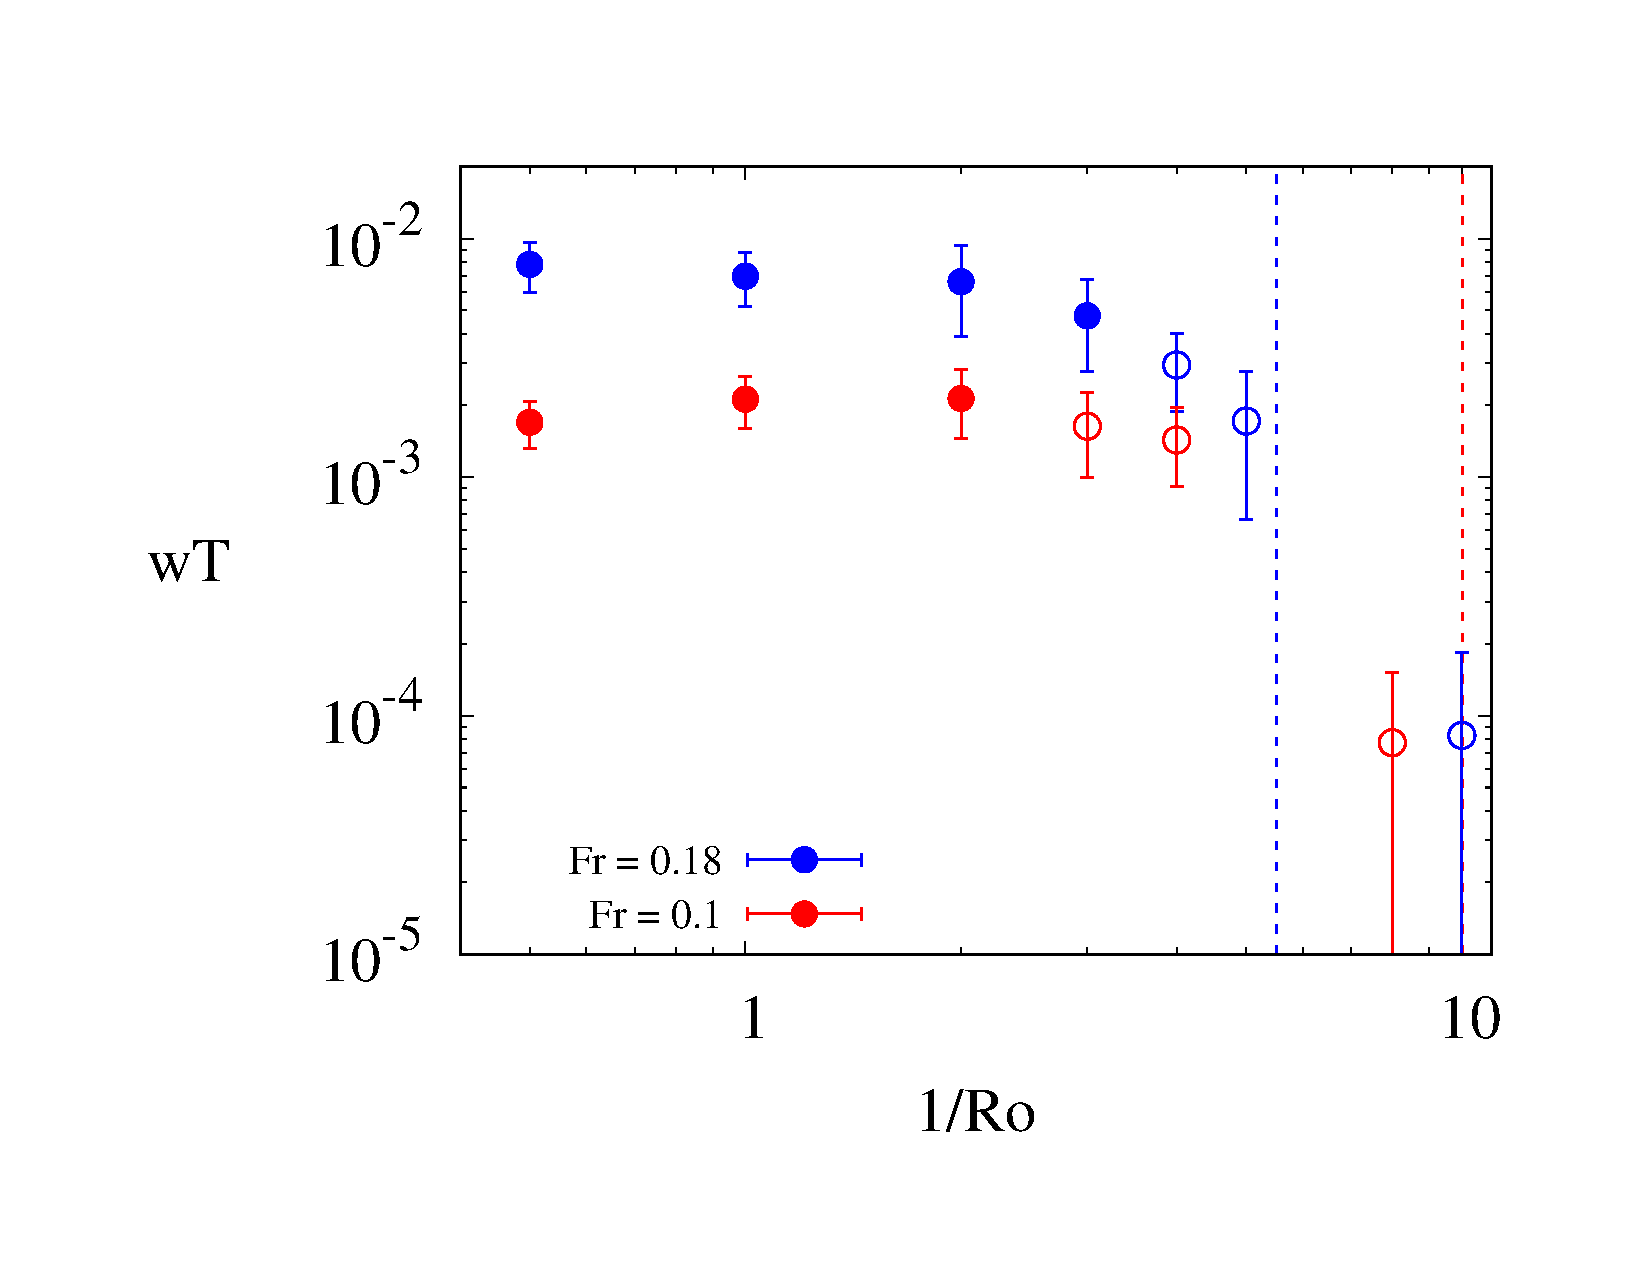
\includegraphics[width=1\textwidth]{images/bflux_plot.pdf}
    \emp

\end{frame}



\begin{frame}{Mixing and Vertical Vorticity}
    \centering
    \bmp{0.07}
        $\omega_z$

        \vspace{75pt}

        $\frac{|\nabla T|^2}{Pe}$
    \emp
    \bmp{0.31}
        \centering
        $1/Ro = 1$
        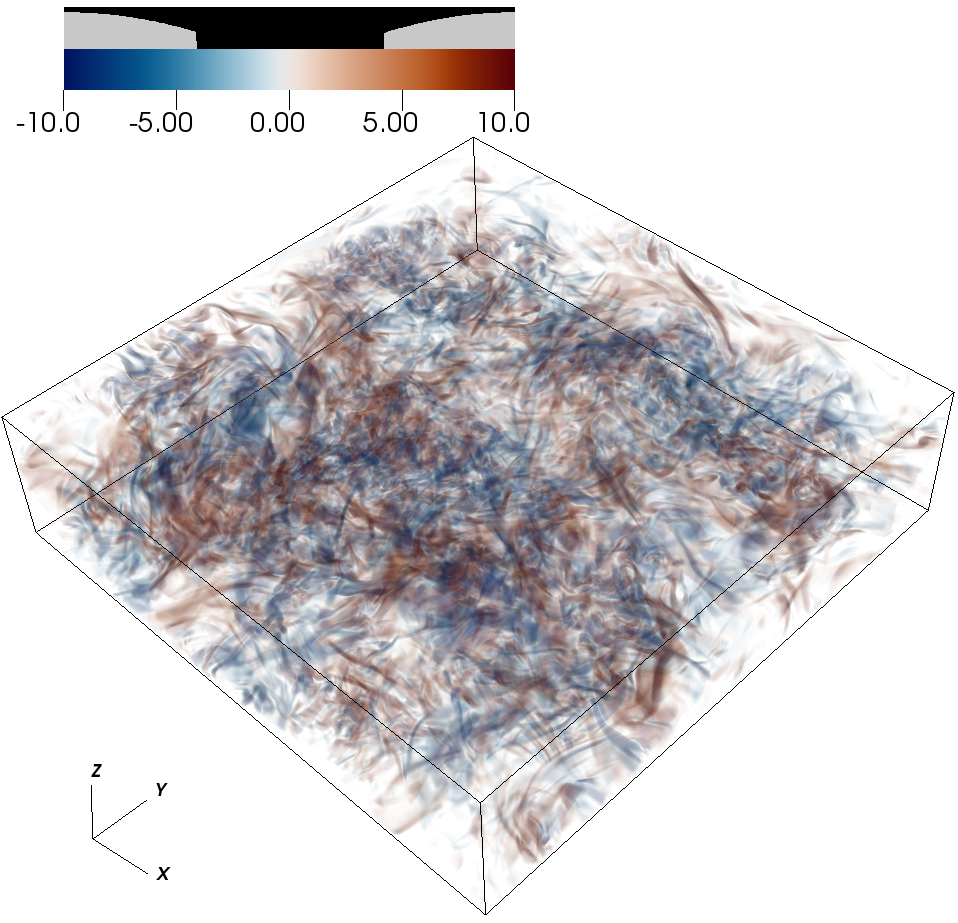
\includegraphics[width=.95\textwidth]{images/vortz_Om0.5_vr2.png}
        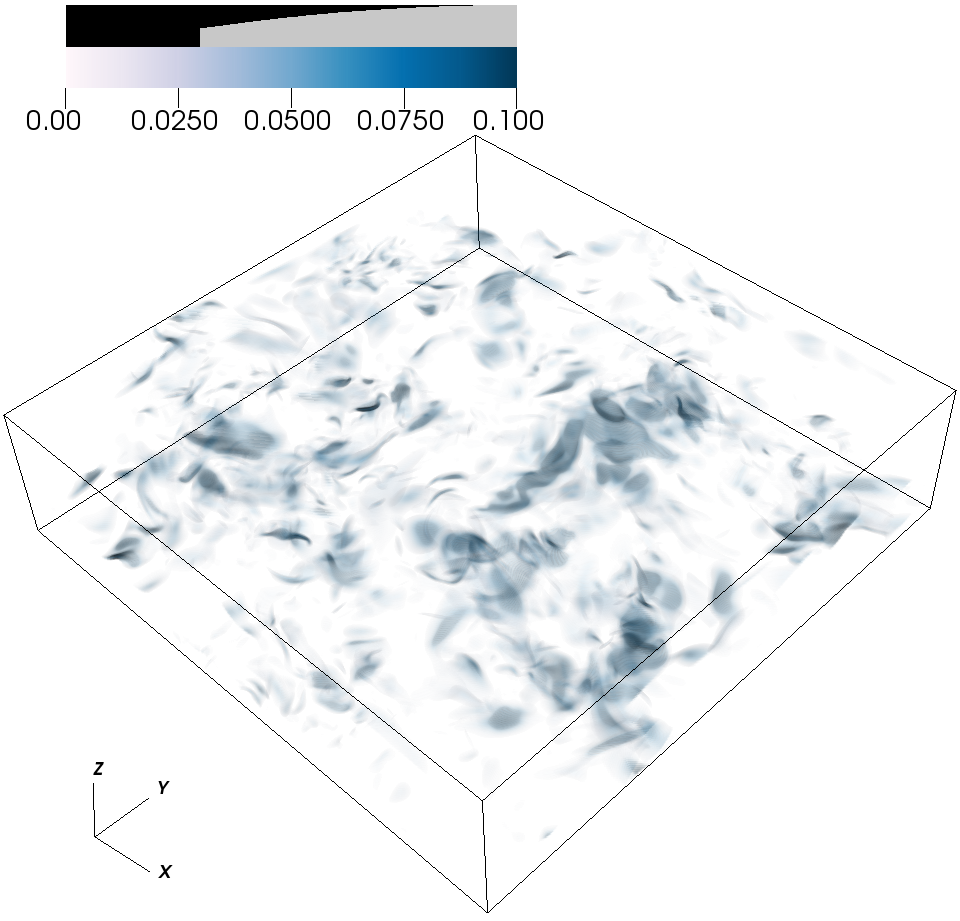
\includegraphics[width=.95\textwidth]{images/chi_Om0.5_vr2.png}
    \emp
    \bmp{0.31}
        \centering
        $1/Ro = 2$
        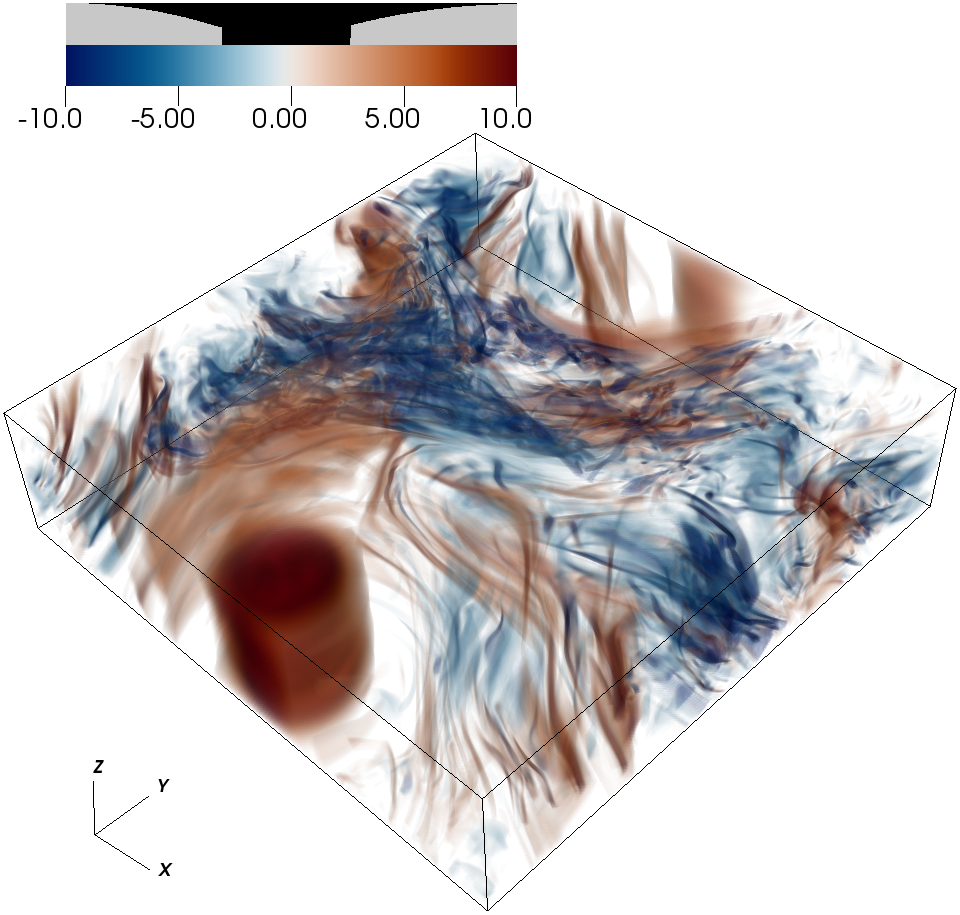
\includegraphics[width=.95\textwidth]{images/vortz_Om2_vr2.png}
        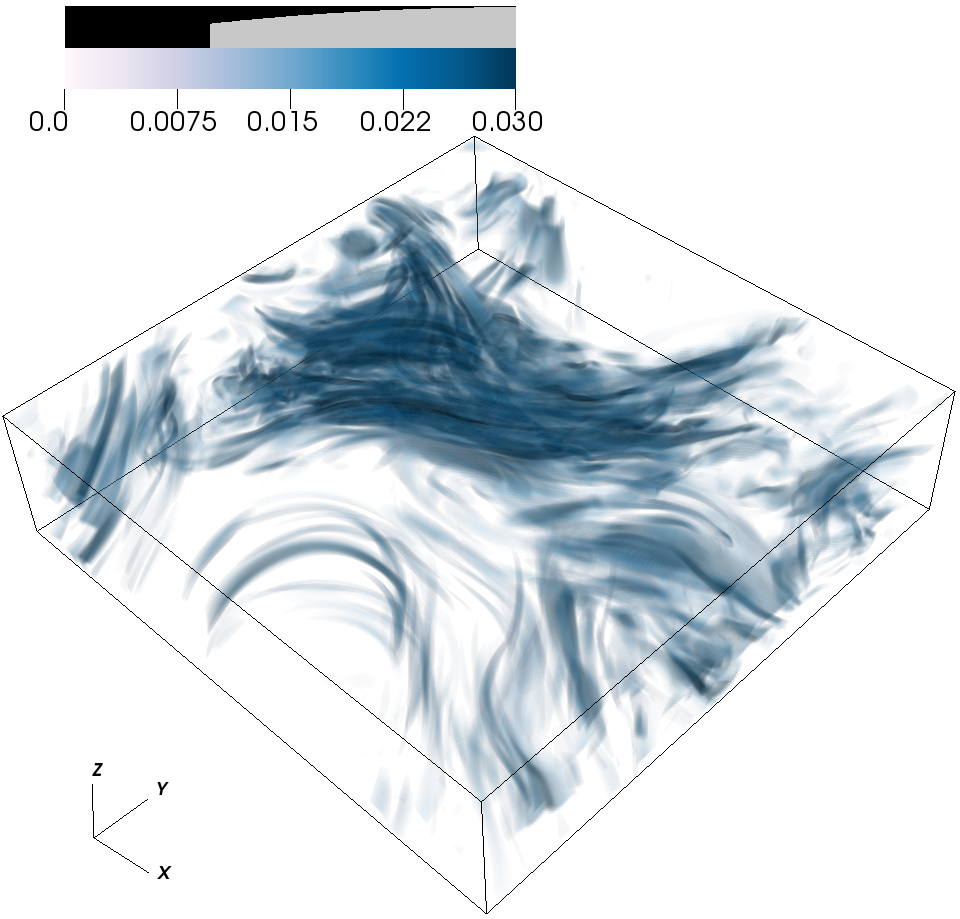
\includegraphics[width=.95\textwidth]{images/chi_Om2_vr2.png}
    \emp
    \bmp{0.31}
        \centering
        $1/Ro = 10$
        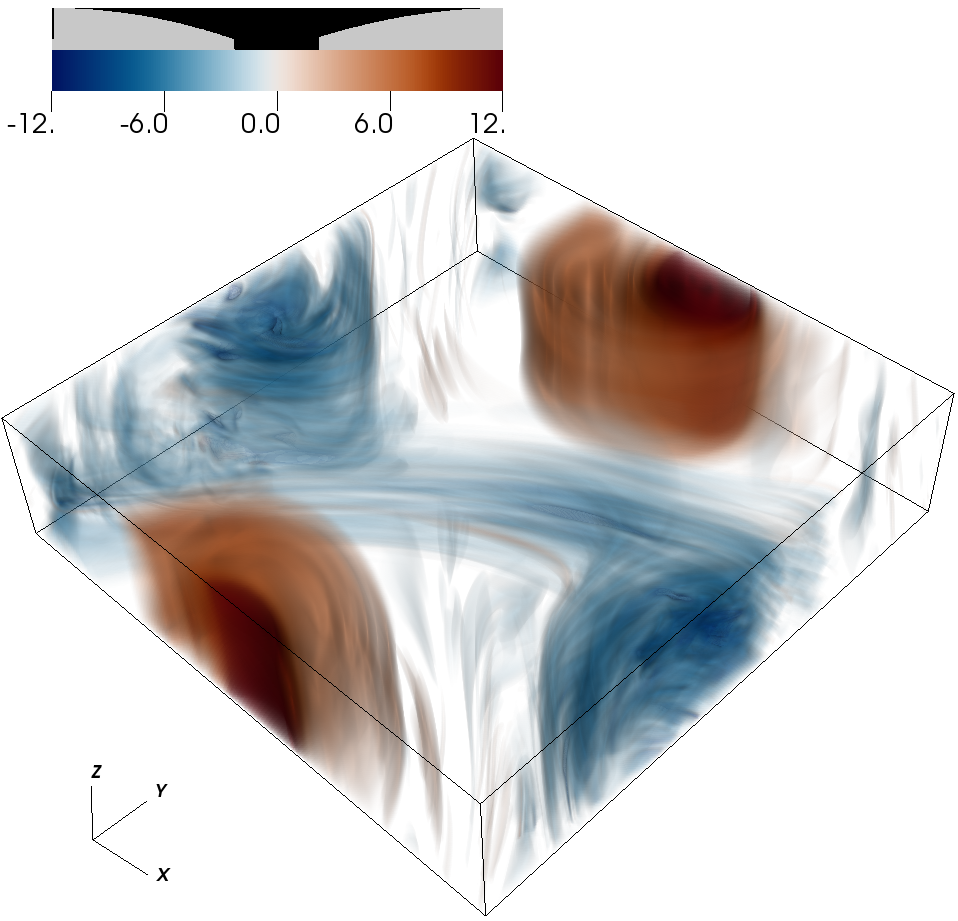
\includegraphics[width=.95\textwidth]{images/vortz_Om10_vr2.png}
        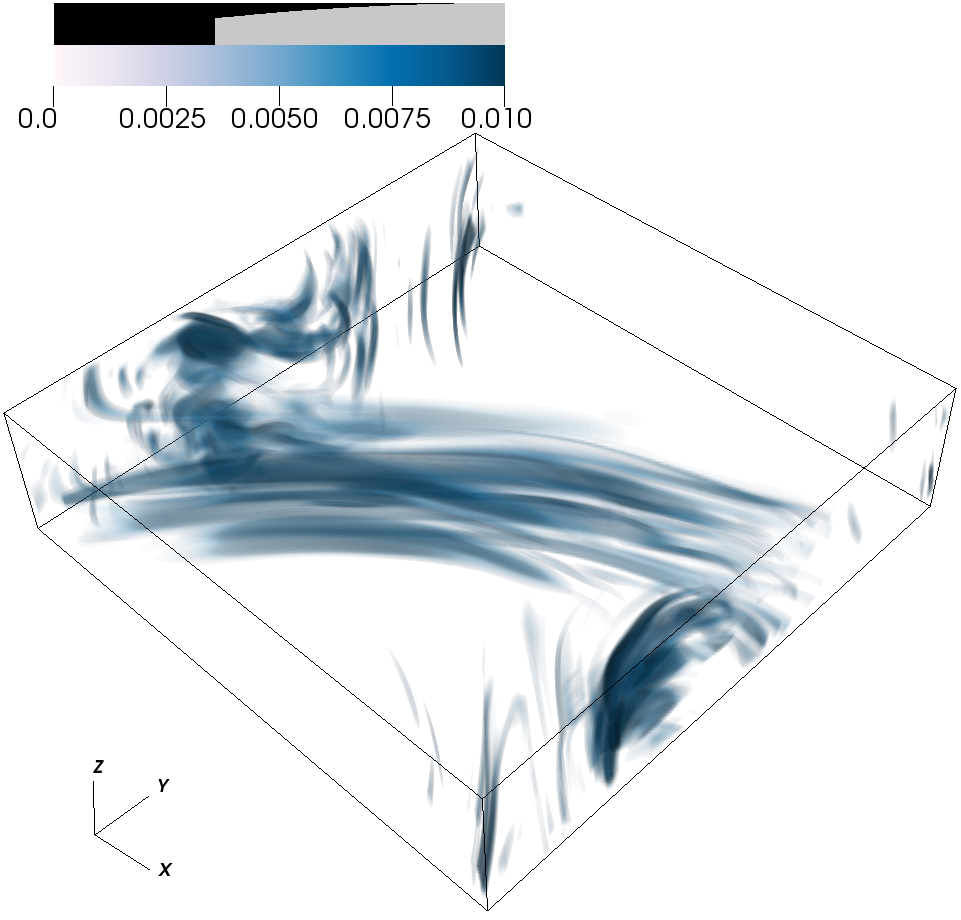
\includegraphics[width=.95\textwidth]{images/chi_Om10_vr2.png}
    \emp


\end{frame}


\begin{frame}{Conclusion}

    \begin{itemize}
        \item Stochastic forcing produces flow with notably different properties compared to steady forcing.
        \item Method of isolating mean and fluctuation dynamics must be modified.
        \item Rapid rotation influences the mean flow before it influences the fluctuations. Vertical mixing is only affected when $Ro \to Fr$
        \item In rapidly rotating flows, mixing is contained in regions of anti-cyclones.
        \item Very rapid rotation inhibits vertical mixing completely.
    \end{itemize}

\end{frame}

{\scriptsize
\bibliographystyle{apj}
\bibliography{BuhlThesis}
}
\end{document}
